In order to evaluate the viability of PIP's c-tables approach to continuous variables, we have implemented an initial version of PIP as an extension to the PostgreSQL DBMS as shown in Figure \ref{fig:blockdiag}.  %PIP's extended functionality is provided by a set of user-defined functions written in C.  

\begin{figure}
\begin{center}
\resizebox{2in}{!}{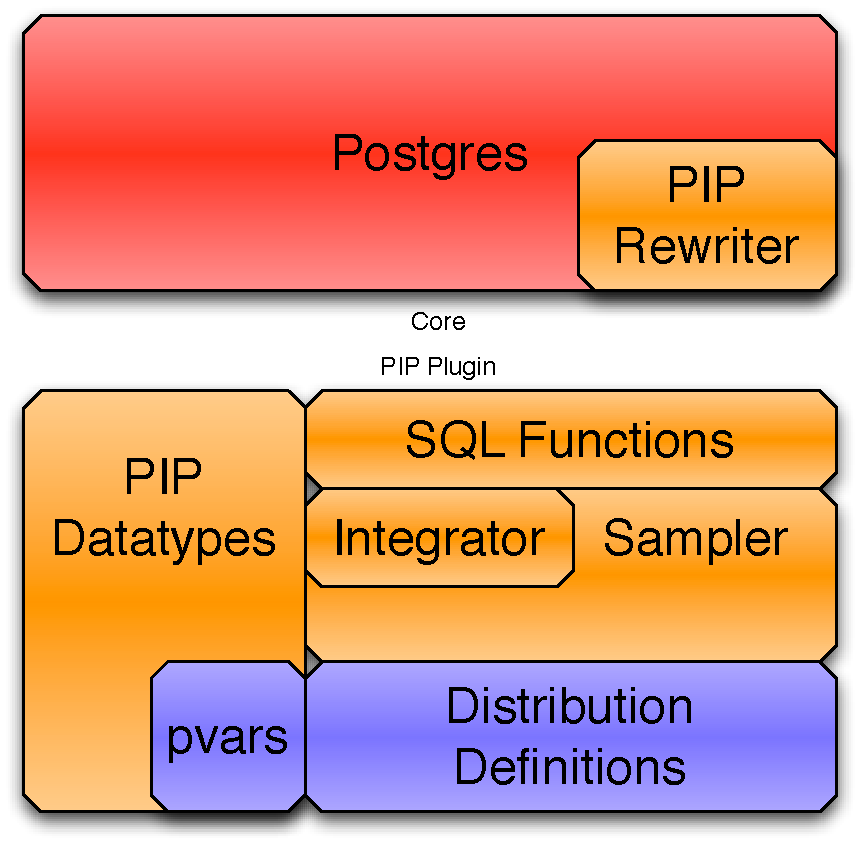
\includegraphics{graphics/blockdiag.pdf}}
\caption{The PIP Postgres plugin architecture}
\label{fig:blockdiag}
\end{center}
\vspace*{-0.3in}
\end{figure}

\subsection{Query Rewriting}
Much of this added functionality takes advantage of PostgreSQL's extensibility features, and can be used ``out-of-the-box".  For example, we define the function 
\[
\mbox{\textbf{CREATE\_VARIABLE($distribution$[,$params$])}}
\]
which is used to create continuous variables\footnote{For discrete distributions, PIP uses a repair-key operator similar to that used in \cite{KochMayBMS2008}}.  Each call allocates a new variable, or a set of jointly distributed variables and initializes it with the specified parameters.  When defining selection targets, operator overloading is used to make random variables appear as normal variables; arbitrary equations may be constructed in this way.  

%\begin{example}\em
%Continuous variables may be created inline with the create-variable operation.  
%
%\begin{verbatim}
%select o.order_id, o.item_id,
%       CREATE_VARIABLE (`Normal', p.mean,
%         p.std_dev) AS delivery_time
%from   orders o, params p
%where  o.item_id = p.item_id;
%\end{verbatim}
%
%\end{example}

%Angle brackets around a random variable are shorthand for the variable's expectation.  All instances of this are replaced by a call to pip's expectation sampling function.  

To complete the illusion, we have modified PostgreSQL itself to add support for C-Table constructs.  Under the modified PostgreSQL when defining a datatype, it is possible to declare it as a CTYPE; doing so has the following three effects:
\begin{itemize}
\item CTYPE columns (and conjunctions of CTYPE columns) may appear in the WHERE and HAVING clauses of a SELECT statement.  When found, the CTYPE components of clause are moved to the SELECT's target clause.  For example, if either $(A>B)$ resolves to a CTYPE variable, 
{\small\begin{verbatim}
  select *
  from   inputs
  where  X>Y and Z like '%foo'
\end{verbatim}}
is rewritten to
{\small\begin{verbatim}
  select *, X>Y
  from   inputs
  where  Z like '%foo'
\end{verbatim}}

\item SELECT target clauses are rewritten to ensure that all CTYPE columns in input tables are passed through.   The exception to this is in the case of special probability-removing functions.  If the select statement contains one or more such functions (typically aggregates, or the conf operator), CTYPE columns are not passed through.  

\item In the case of aggregates, the mechanism by which CTYPE columns may be passed through is unclear.  Thus If the select statement contains an aggregate and one or more input tables have CTYPE columns, the query causes an error unless the aggregate is labeled as a probability-removing function.

\item UNION operations are rewritten to ensure that the number of CTYPE columns in their inputs is consistent.  If one input table has more CTYPE columns of a given type than the other, the latter is padded with NULL constraints.

\end{itemize}

\begin{figure}
\begin{center}
\begin{tabular}{c|ccc}
$R_{ctable}$ & $A$ & $B$ & $\phi$ \\ \hline
& $X*3$ & $5$ & $X > Y \wedge Y > 3$ \\
& $Y$ & $3$ & $Y < 3 \vee X < Y$ \\
\end{tabular}
\begin{center}
$\Downarrow \Downarrow \Downarrow$
\end{center}
\begin{tabular}{c|cccc}
$R_{int}$ & $A$ \begin{footnotesize}(VarExp)\end{footnotesize} & $B$ \begin{footnotesize}(integer)\end{footnotesize} & $\phi_1$ \begin{footnotesize}(CTYPE)\end{footnotesize}& $\phi_2$  \begin{footnotesize}(CTYPE)\end{footnotesize} \\ \hline
& $X*3$ & $5$ & $X > Y$ & $Y > 3$ \\
& $Y$ & $3$ & $Y < 3$ & NULL \\
& $Y$ & $3$ & $X < Y$ & NULL \\
\end{tabular}
\caption{Internal representation of C-Tables}
\label{fig:intrep}
\end{center}
\vspace*{-0.3in}
\end{figure}



Note that these extensions are not required to access PIP's core functionality; they exist to allow users to seamlessly use deterministic queries on probabilistic data.

PIP takes advantage of this by encoding constraint atoms in a CTYPE datatype; Overloaded $>$ and $<$ operators return a constraint atom instead of a boolean if a random variable is involved in the inequality, and the user can ignore the distinction between random variable and constant value (until the final statistical analysis).


\subsection{Defining Distributions}
PIP's primary benefit over other c-tables implementations is its ability to admit variables chosen from arbitrary continuous distributions.  These distributions are specified in terms of general distribution classes, a set of C functions that describes the distribution.  In addition to a small number of functions used to parse and encode parameter strings, each PIP distribution class defines one or more of the following functions.
\begin{itemize}
\footnotesize
\item \texttt{Generate(Parameters, Seed)} uses a pseudorandom number generator to generate a value sampled from the distribution.  The seed value allows PIP to limit the amount of state it needs to maintain; multiple calls to Generate with the same seed value produce the same sample, so only the seed value need be stored.
\item \texttt{PDF(Parameters, x)} evaluates the probability density function of the distribution at the specified point.  
\item \texttt{CDF(Parameters, x)} evaluates the cumulative distribution function at the specified point.
\item \texttt{InverseCDF(Parameters, Value)} evaluates the inverse of the cumulative distribution function at the specified point.
\end{itemize}

PIP requires that all distribution classes define a Generate function.  All other functions are optional, but can be used to improve PIP's performance if provided; The supplemental functions need only be included when known methods exist for evaluating them efficiently.

%Future implementations could conceivably generalize the sampling process.  A sample may be generated using any of the four functions: The Metropolis-Hastings algorithm can sample from an arbitrary PDF, the inverse CDF evaluated on a uniform random value produces a sample, and a binary search may be used to evaluate the inverse CDF given the CDF.

\subsection{Sampling Functionality}
PIP provides several functions for analyzing the uncertainty encoded in a c-table.  The two core analysis functions are conf() and expectation().

\begin{itemize}
\footnotesize
\item \texttt{conf()} performs a conjunctive integration to estimate the probability of a specific row being present in the output, in effect computing the expectation $E[1]$.  It identifies and extracts all lineage atoms from the row being processed and then performs the conjunctive integration over them as normal.

\item \texttt{aconf()}, a variant of conf(), is used to perform general integration.  This function is an aggregate that computes the joint probability of at least one aggregated row being present in the output.  

\item \texttt{expectation()} computes the expectation of a variable by repeated sampling.  If a row is specified when the function is called, the sampling process is constrained by the constraint atoms present in the row.

\item \texttt{expected\_sum()}, \texttt{expected\_max()} are aggregate variants of expectation.  As with expectation() they can be parametrized by a row to specify constraints.

\item \texttt{expected\_sum\_hist()}, \texttt{expected\_max\_hist()} are similar to the above aggregates in that they perform sampling.  However, instead of outputting the average of the results, it instead outputs an array of all the generated samples.  This array may be used to generate histograms and similar visualizations.
\end{itemize}

Aggregates pose a challenge for the query phase of the PIP evaluation process.  Though it is theoretically possible to create composite variables that represent aggregates of their inputs, in practice it is infeasible to do so.  The size of such a composite is not just unbounded, but linear in the size of the input table.  A composite aggregate variable could easily grow to an unmanageable level.  Instead, PIP limits random variable aggregation to the sampling phase.  



